\chapter{The Large Hadron Collider and the \ATLAS Detector}\label{chap:lhc_atlas}

%AB: The work presented in this thesis relies on data recorded by the ATLAS detector in high energy proton-proton collisions. This chapter provides an overview of the experimental apparatus and analysis techniques used throughout this thesis.

The Large Hadron Collider (\LHC) at \CERN has extended the frontiers of particle physics through its unprecedented energy and luminosity.
The \LHC accelerates protons around a \SI{27}{\km} ring until they are travelling just \SI{3}{\m\per\s} slower than than the speed of light, at which point they are made to collide.
The protons travel round the ring 11 thousand times per second in two concentric beams, which are guided by superconducting magnets cooled using liquid helium to \SI{-271.3}{\degreeCelsius} (\SI{1.9}{\kelvin}).
The beams travel in opposite directions and are crossed at four locations so that collisisons between protons can take place.
Around these collision points four specialised detectors, ALICE~\cite{AliceCollaboration_2008}, CMS~\cite{CMS-TDR-08-001}, LHCb~\cite{LHCbCollaboration_2008} and \ATLAS~\cite{PERF-2007-01}, are located to capture information about the products of the collisions.

\begin{comment}
  An overview of the LHC complex is presented in Figure 3.1. Hydrogen gas is ionised using an
  electric field. The first accelerator in the chain, Linac 2, accelerates these protons to 50 MeV. The
  Proton Synchrotron Booster then accelerates the protons to 1.4 GeV, before they are accelerated to
  25 GeV by the Proton Synchrotron. The energy of the beam is further increased to 450 GeV by the
  Super Proton Synchrotron, before it is split into the two beampipes of the LHC. At this final stage,
  the beams are accelerated to an energy of 6.5 TeV (for Run-2) [25, 27]. Proton bunches are spaced
  by 25 ns, with each bunch containing up to 1.1 × 1011 protons.
\end{comment}

The \LHC is operated in ``runs'' during which beams of protons are actively being circulated and collided. Between runs which there are periods of shutdown while the accelerator and detector machinery is maintained and upgraded.
In 2010, the \LHC collided proton bunches, each containing more than $10^{11}$ particles, 20 million times per second, providing \SI{7}{\TeV} proton-proton collisions at instantaneous luminosities of up to \peakLumi.
\runtwo, which began in 2015, increased the the proton-proton collision energy to \SI{13}{\TeV}.
The bunch spacing was also reduced, leading to a collisison rate of \SI{40}{\mega\hertz}.
Over the course of \runtwo a total integrated luminosity of \runtwointlumi was recorded. % less good for physics
2022 marked the beginning of \runthree which, with a higher center of mass energy and peak luminosity, is expected to culminate in the approximate doubling of the dataset size.
%We will be focusing the proton beams at the interaction points to less than 10 micron beam size, to increase the collision rate. (nominal beam size (width) is 16 microns from around run1)

\begin{table}[!htbp]
  \footnotesize\centering
  \setlength{\tabcolsep}{0.5em} % for the horizontal padding
  \begin{tabular}{cc|cccc}
      \toprule 
      \textbf{Period} & \textbf{Year} & $\sqrt{s}$ [\unit\TeV] 
      & \angles{\mu} & \textbf{Bunch spacing} [\unit\ns] & \textbf{Luminosity} [\unit\invcmsqpersec] \\
      \hline
      Run 1 & 2011--2012 & \SIrange[range-phrase=--,range-units=single,range-exponents=combine]{7}{8}{} & 18 & 50 & $8 \times 10^{33}$ \\
      Run 2 & 2015--2018 & \SI{13  }{} & 34 & 25 & $1\textnormal{--}2 \times 10^{34}$ \\
      Run 3 & 2022--2025 & \SI{13.6}{} & 50 & 25 & $2 \times 10^{34}$ \\
      \bottomrule
  \end{tabular}
  \caption{
    Overview of the different LHC runs.
    The average number of interactions per bunch crossing is denoted as \angles{\mu}.
    Numbers for Run 3 are preliminary and are only provided to give an indication of expected performance.
    Also show integrated luminosity?
    Do I need to cite public plots?
    % run 1 run 2 trigger https://cds.cern.ch/record/2058218/
    %https://twiki.cern.ch/twiki/bin/view/AtlasPublic/LuminosityPublicResults
    %https://twiki.cern.ch/twiki/bin/view/AtlasPublic/LuminosityPublicResultsRun2
    %  2-3 × 1034 cm−2 s−1 and an average pileup of ~80 collisions/bunch crossing
    % https://cds.cern.ch/record/2732959/files/LHCP2020_094.pdf
  }
  \label{tab:lhc_runs}
\end{table}


\section{Collider Definitions \& Coordinate Systems}
The luminosity is defined by
%
\begin{equation}\label{eq:lumi_def}
L = \frac{1}{\sigma} \der{N}{t} ,
\end{equation}
%
where $N$ is the number of individual proton-proton collisions and $\sigma$ is the cross-sectional area of the beams as they cross.

\begin{itemize}
  \item transverse/longitudinal planes
  \item rapitidy pseudorapidity etc
\end{itemize}


\section{The ATLAS Detector}\label{sec:atlas_detector}

%% from https://twiki.cern.ch/twiki/bin/view/AtlasProtected/PubComCommonText
% Footnote with ATLAS coordinate system
\newcommand{\AtlasCoordFootnote}{%
ATLAS uses a right-handed coordinate system with its origin at the nominal interaction point in the centre of the detector and the \axis{z} along the beam pipe. The \axis{x} points from the interaction point to the centre of the LHC ring, and the \axis{y} points upwards. Cylindrical coordinates \((r,\phi)\) are used in the transverse plane, \(\phi\) being the azimuthal angle around the \axis{z}. The pseudorapidity is defined in terms of the polar angle \(\theta\) as \(\eta = -\ln \tan(\theta/2)\). Angular distance is measured in units of \(\DeltaR \equiv \sqrt{(\Delta\eta)^{2} + (\Delta\phi)^{2}}\).}

The ATLAS\footnote{A Toroidal Lhc ApparatuS.} detector at the LHC covers nearly the entire solid angle around the collision point.\footnote{\AtlasCoordFootnote}
It consists of an inner tracking detector surrounded by a thin superconducting solenoid, electromagnetic and hadronic calorimeters,
and a muon spectrometer incorporating three large superconducting air-core toroidal magnets.\todo{okay this is the standard pubcom text?}

The detector is made up of several specialised sub-detectors as shown in \cref{fig:atlas_detector}.
In this section a condensed overview of each sub-detector is given, in order of increasing radial distance from the point of collision.
A more complete picture can be found in \rcite{PERF-2007-01}, or in the technical design reports (TDRs) of the individual sub-detectors.

\begin{figure}[!htpb]
  \centering
  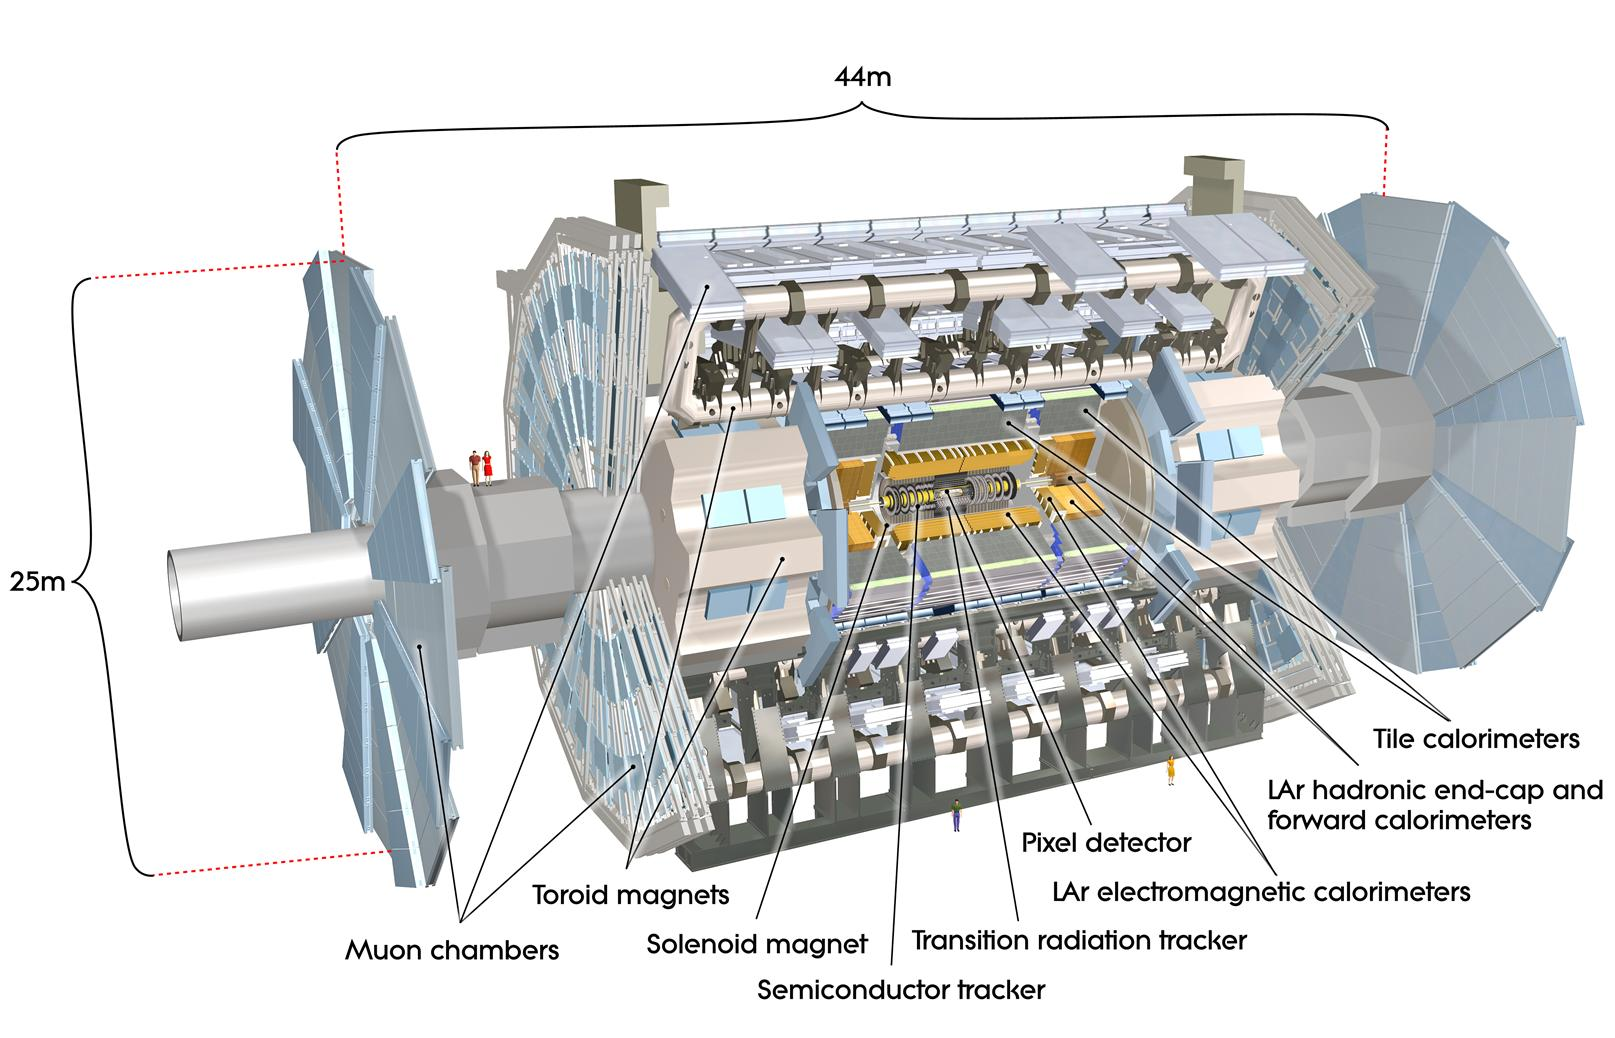
\includegraphics[width=0.85\linewidth]{chapters/2.detector/figs/atlas_detector.jpg}
  \caption{The \ATLAS detector. Cutouts are shown}
  \label{fig:atlas_detector}
\end{figure}
%


\subsection{The Inner Detector}\label{sec:atlas_id}

The inner-detector system (ID) provides high-resolution charged-particle trajectory tracking in the range $|\eta| < 2.5$.
The ID is immersed in a \SI{2}{\tesla} axial magnetic field, produced by a superconducting solenoidal magnet, which enables the measurement of particle transverse momentum and charge\footnote{Reconstructed charged particles are assumed to have a charge of $\pm 1$.}.
% Momentum resolution is sufficient to identify the charge sign of particles up to the highest energies expected at LHC.
After \runthree, the ID will be replaced by the ITk \cite{CERN-LHCC-2017-021}.

The inner detector is made up of several sub-systems, shown in \cref{fig:atlas_id_run1,fig:atlas_id_run2}.
The high-granularity silicon pixel detector covers the vertex region and typically provides four spacepoint measurements per track.
It is followed by the silicon microstrip tracker (SCT), which usually provides a further four spacepoint measurements per track.
These silicon detectors are complemented by the transition radiation tracker (TRT),
which enables radially extended track reconstruction up to \(|\eta| = 2.0\). 


\begin{figure}[!htpb]
  \centering
  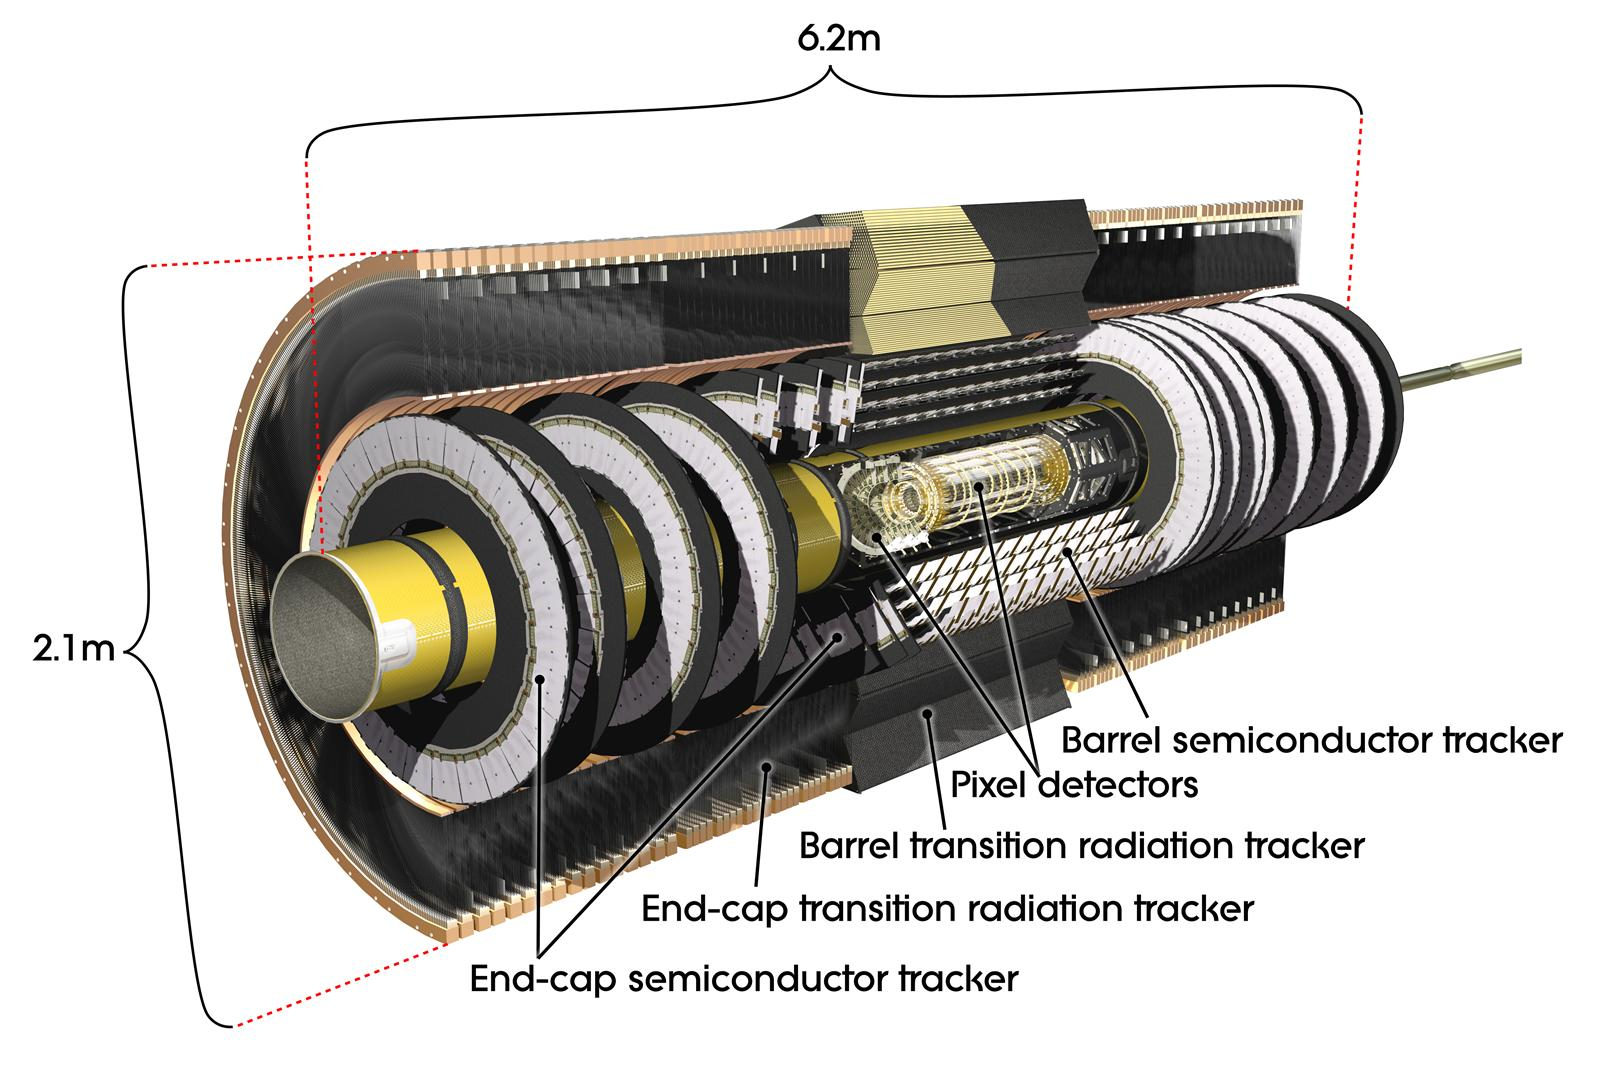
\includegraphics[width=0.7\linewidth]{chapters/2.detector/figs/atlas_id.jpg}
  \caption{A 3D model of the \ATLAS ID showing the barrel layers and end-cap disks.}
  \label{fig:atlas_id_run1}
\end{figure}

\begin{figure}[!htpb]
  \centering
  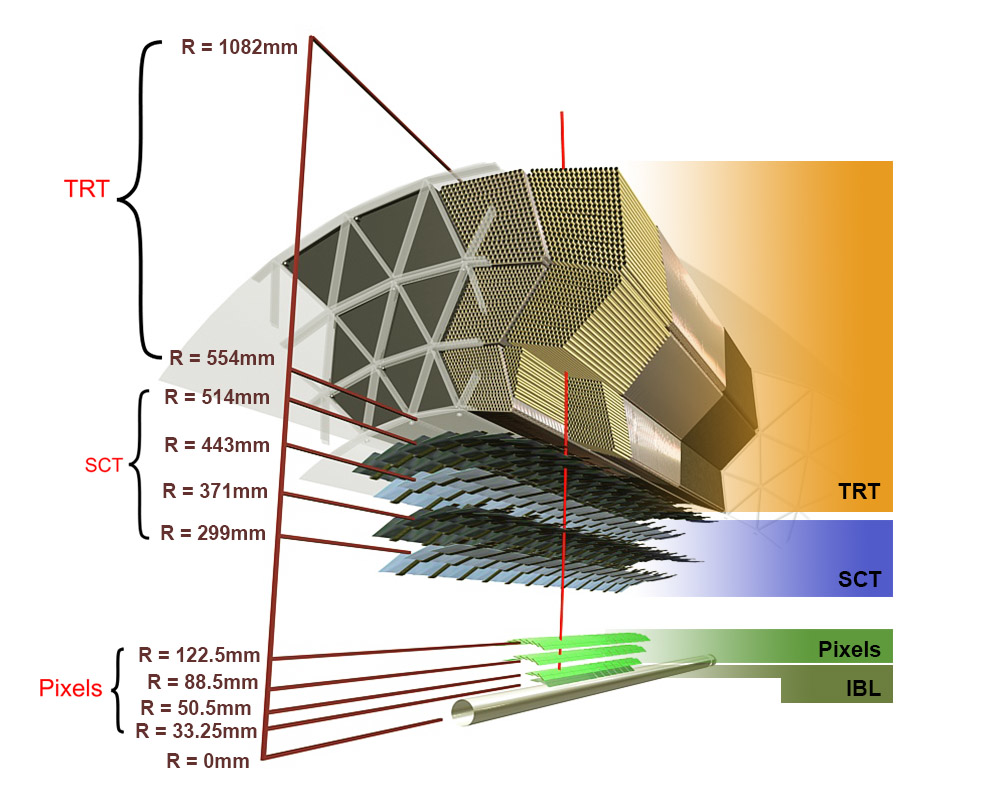
\includegraphics[width=0.75\linewidth]{chapters/2.detector/figs/atlas_id_xs.png}
  \caption{A cross-sectional view of the \ATLAS ID showing the radii of the different detector layers.}
  \label{fig:atlas_id_run2}
\end{figure}


\subsubsection{Pixel Detector}
The silicon pixel detector is comprised of four cylindrical barrels at increasing radii from the beamline, and four disks on each side.
The innermost barrel layer is the insertable B-layer (IBL), which was installed before \runtwo \cite{ATLAS-TDR-19,PIX-2018-001}.
%Radiation-hard electronics are used to read out the 140 million channels.
The specification of the pixel detector determines the impact parameter resolution and the ability to reconstruct primary and secondary vertices.
The detector is required to have a high granularity (i.e. resolution) to maintain the low occupancy required to resolve nearby particles. %(high sparsity to resolve different tracks).
Individual pixels are \SI{50}{\micro\meter} in the transverse direction $R\phi$ and \SI{400}{\micro\meter} in the longitudinal $z$ direction (\SI{250}{\micro\meter} for the IBL).
Cluster positions have a resolution of approximately \SI{10}{\micro\meter} in $R\phi$ and \SI{100}{\micro\meter} in $z$.

%giving a resolution of 10 µm in the transverse direction and 115 µm in the longitudinal direction in the barrel region.
%For the IBL, pixels are \SI{50}{\micro\meter} in the $R\phi$ direction and \SI{250}{\micro\meter} in the $z$ direction, giving a cluster resolution of 10 µm in the transverse direction and 115 µm in the longitudinal direction in the barrel region.
%%Pixel clusters and provide an Xlocal resolution of about 10 µm, depending on the particle incident angle

\begin{figure}[!htpb]
  \centering
  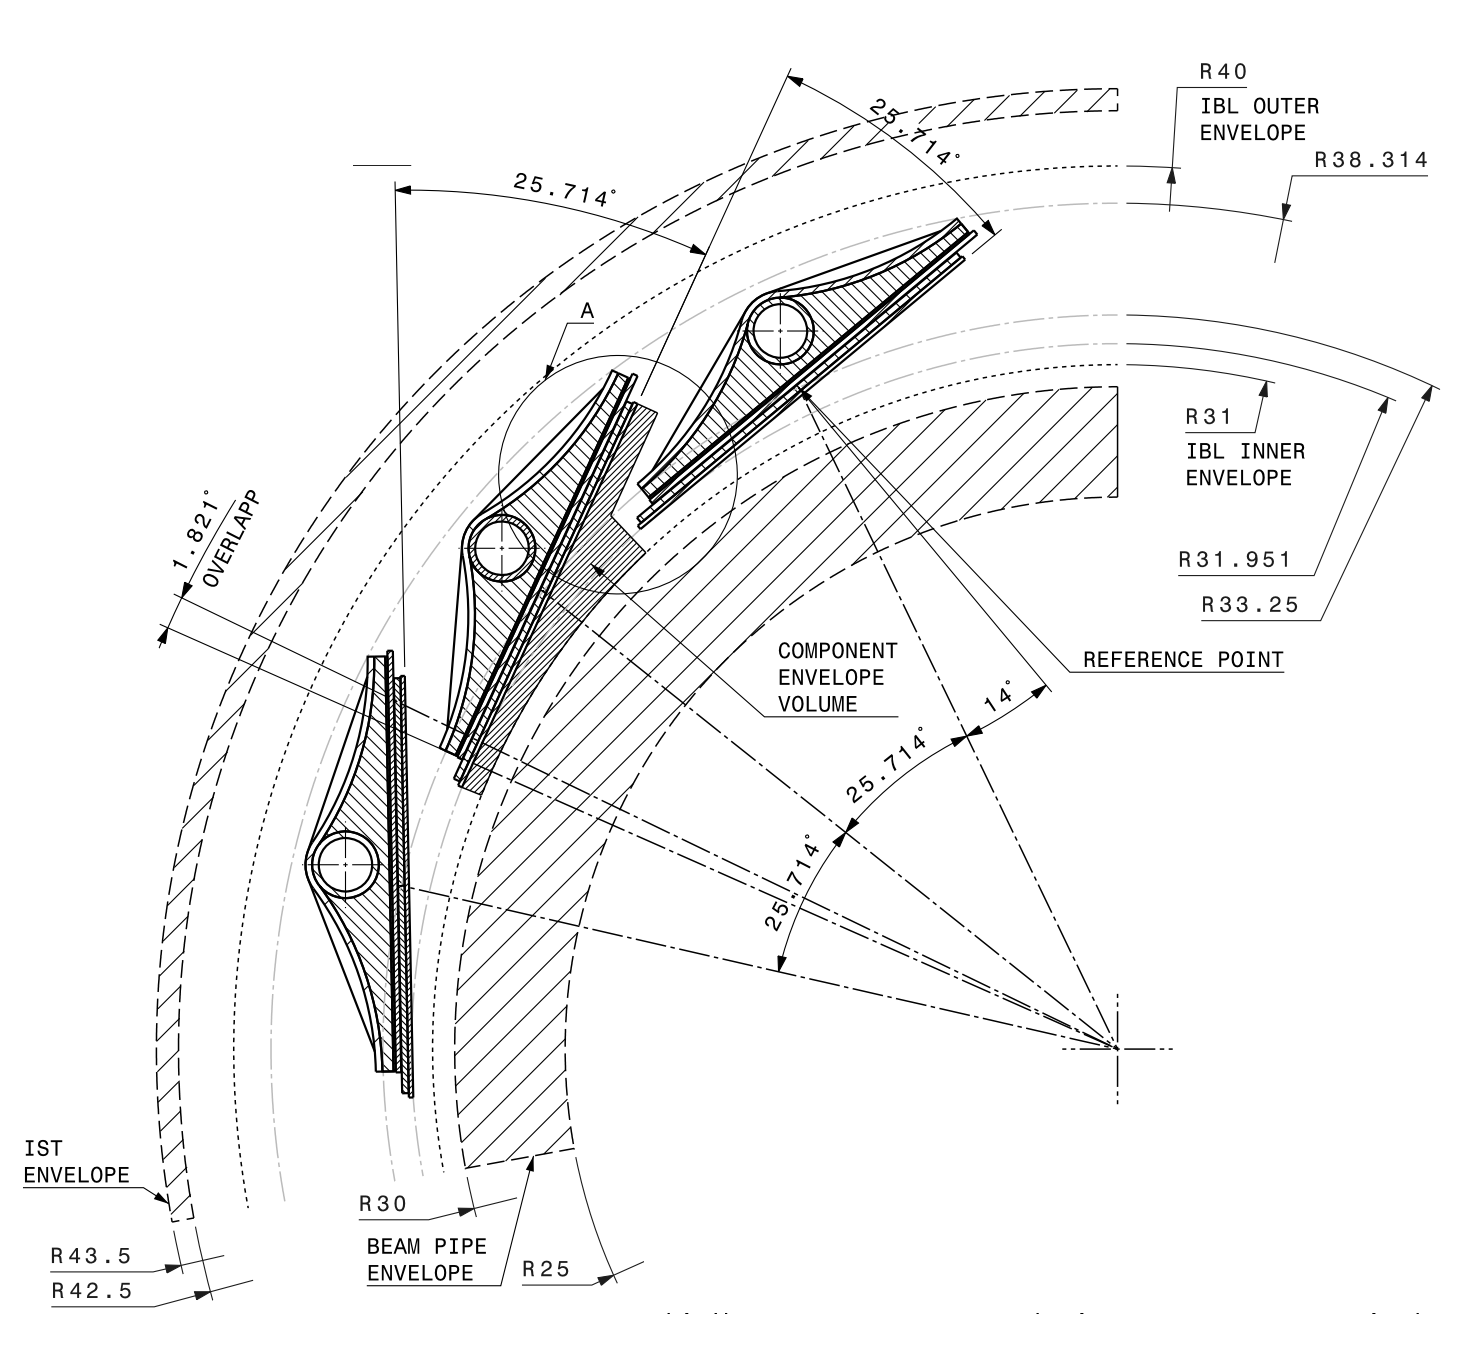
\includegraphics[width=0.6\linewidth]{chapters/2.detector/figs/atlas_ibl.png}
  \caption{A cross-sectional view of the \ATLAS IBL.}
  \label{fig:atlas_ibl}
\end{figure}

\subsubsection{Semi-Conductor Tracker (SCT)}
The SCT is made up of four concentric barrel layers in the central region, and nine disks in each end-cap.
Each layer is itself made of a pair of silicon microstrip layers, with a small stereo angle (\SI{20}{\milli\radian}) between the two layers enabling the $z$\nobreakdash-coordinate measurement from a pair of strip measurements.
The SCT typically provides four precision spacepoint measurements (eight strip measurements) per track in the barrel region.
These have intrinsic uncertainties of \SI{17}{\micro\meter} in the transverse direction $R\phi$, and \SI{580}{\micro\meter} in the longitudinal direction $z$.
The measurements provide a key contribution to the measurement of charged-particle momentum and impact parameter, along with vertex position.
%The high granularity enables good pattern recognition
Charge-particle tracks can be distinguished if separated by more than $\sim \SI{200}{\micro\meter}$.
Hits are registered as binary signals if the pulse height in a channel exceeds a certain threshold.


\subsubsection{Transition Radiation Tracker (TRT)}
The TRT is a straw-tube tracker which complements the higher-resolution silicon-based tracks by offering a larger number of hits per track (typically around 30) and a long lever arm, which aids the accurate measurement of particle momentum. 
It is made up of approximately \num{300000} drift tubes with a diameter of \SI{4}{\milli\meter} which are filled with xenon gas.
The walls of each tube are electrically charged, and a thin conducting wire runs along the center.
When a charged particle traverses a tube, it ionises the xenon and the resulting liberated electrons drift along the electric field to the wire, where an associated charge is registered.
In the barrel the straws run parallel to the \axis{z} and therefore the TRT only provides tracking information in $R\phi$. Straws are arranged radially in the end-caps. The resulting two-dimensional spacepoints have a resolution of approximately \SI{120}{\micro\meter}.
The spaces between the straws are filled with a polymer which leads to the emission of transition radiation, aiding electron identification.

%It allows the ID to reconstruct $V_0$s which are especially interesting in CP-violating $B$ decays.
%Electron identification capability is added by employing xenon gas to detect transition-radiation photons created in a radiator between the straws. In addition it provides additional discrimination between electrons and hadrons
% provides electron identification information based on the fraction of hits (typically 30 in total) above a higher energy-deposit threshold corresponding to transition radiation.
%may be emitted by highly relativistic charged particles as they traverse a material boundary. This effect depends on the relativistic factor γ = E/m and is strongest for electrons, 
%means it can be used for particle identification (section 6). Typical photon energies are 5–30 keV. These soft X-rays can be absorbed by Xe atoms, depositing additional energy in the gas and leading to significantly higher readout signals. Suc

%Within the radial space available, the straw spacing has been optimised for tracking at the expense of electron identification, which would be improved by a greater path length through the radiator material and fewer active straws. 




\subsection{Calorimeters}\label{sec:calorimeter}

The calorimeter system measures the energy of incident particles over the range $|\eta| < 4.9$.
There are two main sub-systems: the electromagnetic calorimeter (ECal), which focuses on the measurement of electrons and photons, and the hadronic calorimeter (HCal), which measures the energy of hadrons.
Upon entering the calorimeter, incident particles will interact with the detector material to produce a shower of secondary particles with reduced energies. 
The charge deposited in this process is measured to reconstruct the energy of the initial incident particle.
The two calorimeter sub-systems must must provide strong containment of showering particles to prevent punch-through of EM and non-muon particles to the HCal and muon system respectively.

%the fine granularity of the EM calorimeter is ideally suited for precision measurements of electrons and photons. The coarser granularity of the rest of the calorimeter is sufficient to satisfy the physics requirements for jet reconstruction and $E_T^{\textrm{miss}}$ measurements.     

%A narrow transverse profile is characteristic of an electromagnetic cascade. Hadrons passing through matter also initiate cascades through inelastic hadron-nuclei interactions. The shower produces secondary hadrons and leptons and has a comparatively wide transverse profile. 

%Nuclear interaction length is the mean distance travelled by a hadronic particle before undergoing an inelastic nuclear interaction.
%The nuclear interaction length is about an order of magnitude greater than the radiation length of the material. Therefore, like most general purpose experiments, ATLAS uses two different calorimetry systems to measure electrons and photons (the ECal) and hadrons (the HCal). 

%
\begin{figure}[!htpb]
  \centering
  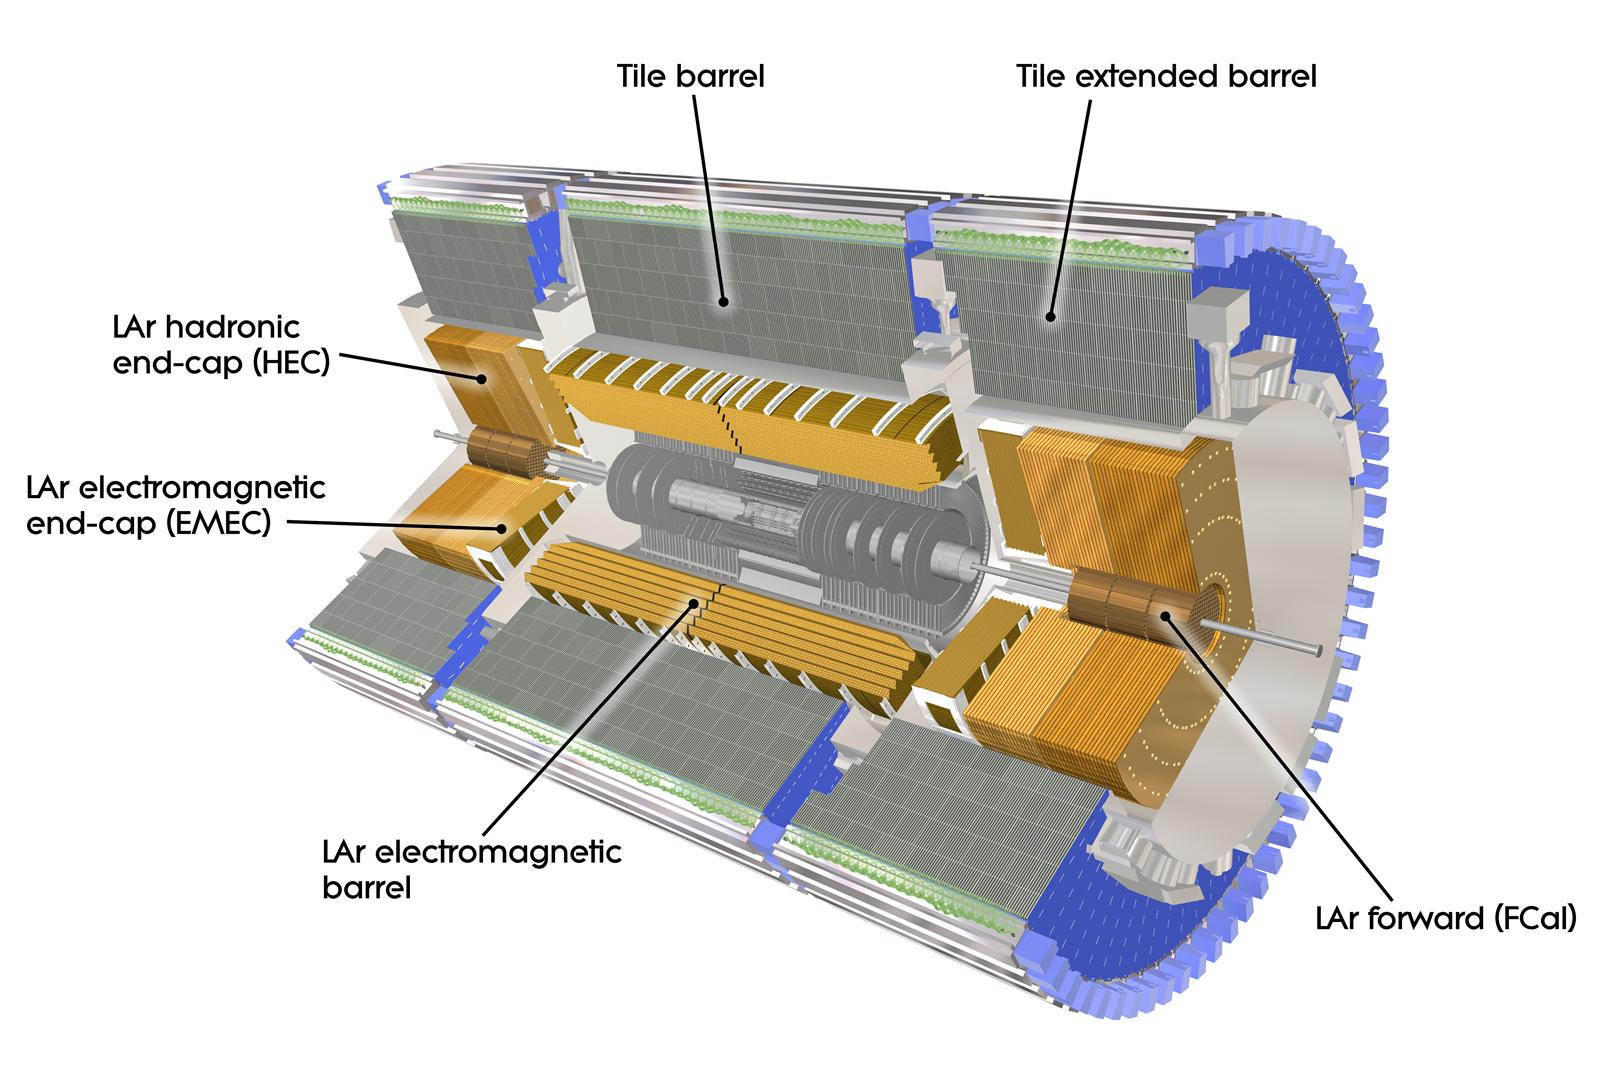
\includegraphics[width=0.8\linewidth]{chapters/2.detector/figs/atlas_calos.jpg}
  \caption{The \ATLAS calorimeters. The ECal (orange) and HCal (grey, brown).}
  \label{fig:atlas_calos}
\end{figure}
%


\subsubsection{Liquid Argon (LAr) Electromagnetic Calorimeter}
The more granular lead/liquid-argon ECal covers the region $|\eta|< 3.2$ and is split into barrel (covering $|\eta| < 1.475$) and end-cap (covering $1.375 < |\eta| < 3.2$) regions.
EM calorimetry works by encouraging electrons and photons to interact with electrically charged particles in detector material via bremsstrahlung ($e \rightarrow e\gamma$) and pair production ($\gamma \rightarrow e^+ e^- $).
The EM calorimeter uses lead absorber plates to initiate EM showers, resulting in secondary particles which ionise the surrounding liquid argon.
The charge is collected on copper electrodes and read out.
The accordion geometry of the ECal allows for a full coverage in $\phi$ without any azimuthal cracks. 

%it initiates an electromagnetic cascade,
%The fine granularity of the EM calorimeter
%Additionally, multiple samplings of the shower are used to resolve its pointing vector.

\subsubsection{Hadronic Tile Calorimeter}
In the central barrel region with $|\eta| < 1.7$, the HCal uses a tile calorimeter with steel as an absorbing material, and scintillating tiles as the active material.
Two copper/liquid-argon calorimeter end-caps are also used.
Incident hadrons interact via the strong and electromagnetic forces with the absorber material, mainly loosing energy due to multiple inelastic nuclear collisions.
The active material captures the resulting electrons and photons to measure the energy of the incident hadron.

%Hadrons are relatively massive and cannot radiate much of their energy through bremsstrahlung, and they lose their energy mainly through multiple nuclear collisions.  Hadrons passing through matter also initiate cascades through inelastic hadron-nuclei interactions.

%The tile calorimeter is placed directly outside the EM calorimeter envelope.o 
%The barrel covers the region -1.0<η<1.0, and the extended barrels cover the region 0.8<|η|<1.7.

%LAr hadronic end-cap calorimeter (HEC). Located directly behind (in $z$) the end-cap electromagnetic calorimeter and sharing the same LAr cryostats. The high level of radiation in the forward regions would cause severe damage to plastic scintillators. In the end-caps, parallel copper plates are submerged in liquid argon, which is preferred as the active medium because of its inherent radiation hardness.


\subsection{Muon System}\label{sec:muon_sys}

The muon spectrometer (MS) comprises separate trigger and
high-precision tracking chambers measuring the deflection of muons in a magnetic field generated by the superconducting air-core toroidal magnets.
The field integral of the toroids ranges between \num{2.0} and \SI{6.0}{\tesla\metre}
across most of the detector. 
Three layers of precision chambers, each consisting of layers of monitored drift tubes, covers the region \(|\eta| < 2.7\),
complemented by cathode-strip chambers in the forward region, where the background is highest.
The muon trigger system covers the range \(|\eta| < 2.4\) with resistive-plate chambers in the barrel, and thin-gap chambers in the end-cap regions.

Based on the magnetic deflection of muon tracks in the large superconducting air-core toroid magnets, instrumented with separate trigger and high-precision tracking chambers. This magnet configuration provides a field which is mostly orthogonal to the muon trajectories, while minimising the degradation of resolution due to multiple scattering. In the barrel region, tracks are measured in chambers arranged in three cylindrical layers around the beam axis; in the transition and end-cap regions, the chambers are installed in planes perpendicular to the beam, also in three layers.

%
\begin{figure}[!htpb]
  \centering
  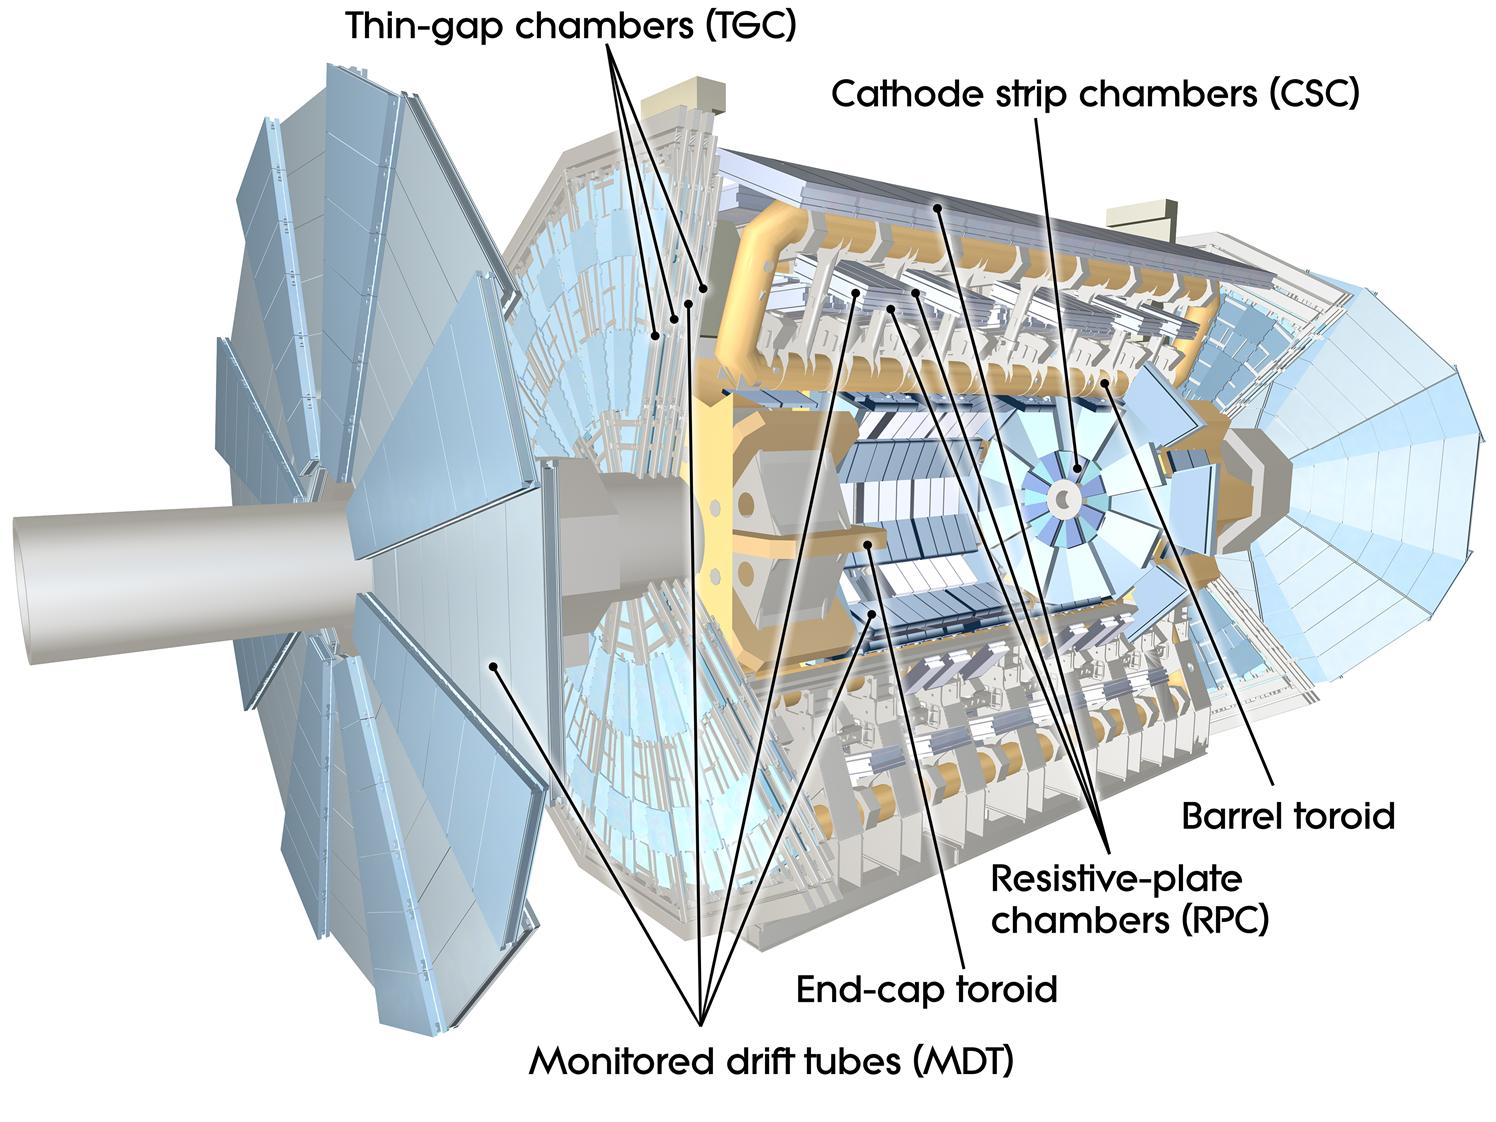
\includegraphics[width=0.4\linewidth]{chapters/2.detector/figs/atlas_muon_system.jpg}
  \caption{The \ATLAS muon detectors.}
  \label{fig:atlas_muon_system}
\end{figure}
%


\subsection{The Trigger}\label{sec:trigger}
An LHCb trigger table borrowed from \texttt{hepthesis} is shown in \TableRef{tab:bg-theory:trigger_details}:

\begin{table}[bht]
  \footnotesize\centering
  \setlength{\tabcolsep}{0.5em} % for the horizontal padding
  \caption{Characteristics of the trigger levels and offline analysis.}
  \begin{tabular}{lllll}
                & L0              & L1              & HLT             \\
    \midrule
    Input rate  & \SI{40}{\MHz} & \SI{1}{\MHz}  & \SI{40}{\kHz} \\
    Output rate & \SI{1}{\MHz}  & \SI{40}{\kHz} & \SI{2}{\kHz}  \\
    Location    & On detector     & Counting room   & Counting room   \\
  \end{tabular}
  \label{tab:bg-theory:trigger_details}
\end{table}


\subsubsection{Triggers and Data Acquisition (TDAQ)}







Interesting events are selected by the first-level trigger system implemented in custom hardware,
followed by selections made by algorithms implemented in software in the high-level trigger~\cite{TRIG-2016-01}. 
The first-level trigger accepts events from the \SI{40}{\MHz} bunch crossings at a rate below \SI{100}{\kHz},
which the high-level trigger further reduces in order to record events to disk at about \SI{1}{\kHz}.

An extensive software suite~\cite{ATL-SOFT-PUB-2021-001} is used in the reconstruction and analysis of real
and simulated data, in detector operations, and in the trigger and data acquisition systems of the experiment.


The trigger system has three distinct levels: L1, L2, and the event filter. Each trigger level refines the decisions made at the previous level and, where necessary, applies additional selection criteria. The data acquisition system receives and buffers the event data from the detector-specific readout electronics, at the L1 trigger accept rate. The first level uses a limited amount of the total detector information to make a decision in in a short time.


\subsubsection{The Trigger System}

The L1 trigger searches for high transverse-momentum muons, electrons, photons, jets, and $\tau$-leptons decaying into hadrons, as well as large missing and total transverse energy. Its selection is based on information from a subset of detectors. High transverse-momentum muons are identified using trigger chambers in the barrel and end-cap regions of the spectrometer. Calorimeter selections are based on reduced-granularity information from all the calorimeters. Results from the L1 muon and calorimeter triggers are processed by the central trigger processor, which implements combinations of different trigger selections. In each event, the L1 trigger also defines one or more Regions-of-Interest (RoI’s), i.e. the geographical coordinates in $\eta$ and $\phi$, of those regions within the detector where its selection process has identified interesting features. The RoI data include information on the type of feature identified and the criteria passed, e.g. a threshold. This information is subsequently used by the high-level trigger.

The L2 selection is seeded by the RoI information provided by the L1 trigger. L2 selections use, at full granularity and precision, all the available detector data within the RoI’s (approximately 2\% of the total event data). The L2 menus are designed to reduce the trigger rate to approximately 3.5 kHz, with an event processing time of about 40 ms, averaged over all events. The final stage of the event selection is carried out by the event filter, which reduces the event rate to roughly 200 Hz. Its selections are implemented using offline analysis procedures within an average event processing time of the order of four seconds.








\section{Reconstructed Physics Objects}\label{sec:physics-objects}

\subsection{Tracks}\label{sec:tracks}

The trajectories of charged particles are reconstructed as tracks from the energy depositions (hits) of the particles as they traverse the sensitive elements of the inner detector.
Track selection follows the loose selection described in Ref.~\cite{ATL-PHYS-PUB-2020-014} and outlined in~\cref{tab:track_selections}, which was found to improve the flavour tagging performance compared to previous tighter selections, whilst ensuring good resolution of tracks and a low fake rate~\cite{PERF-2015-08}.
The transverse IP $d_0$ and longitudinal IP $z_0$ are measured with respect to the hard scatter primary vertex, defined as the reconstructed primary vertex (PV) with the largest sum of the transverse momentum ($\pt$) of the associated tracks squared, $\sum \pt^2$.
%The reconstructed tracks are required to satisfy the quality requirements in \cref{tab:track_selections}.

\begin{table}[!htbp]
  \footnotesize\centering
  \setlength{\tabcolsep}{0.5em} % for the horizontal padding
  \caption{
    Quality selections applied to tracks,
    where $d_0$ is the transverse IP of the track, $z_0$ is the longitudinal IP with respect to the PV and $\theta$ is the track polar angle.
    Shared hits are hits used on multiple tracks which have not been classified as split by the cluster-splitting neural networks~\cite{PERF-2015-08}.
    Shared hits on pixel layers are given a weight of 1, while shared hits in the SCT are given a weight of 0.5.
    A hole is a missing hit, where one is expected, on a layer between two other hits on a track.
    }
  \begin{tabular}{ll}
    \toprule 
    \textbf{Parameter} & \textbf{Selection} \\
    \hline
    $\pt$                & $> 500$ MeV \\
    $|d_0|$              & $< 3.5$ mm \\
    $|z_0 \sin\theta|$   & $< 5$ mm \\
    Silicon hits         & $\ge 8$ \\
    Shared silicon hits  & $< 2$ \\
    Silicon holes        & $< 3$ \\
    Pixel holes          & $< 2$ \\
    \bottomrule
  \end{tabular}
  \vspace{4mm}
  \label{tab:track_selections}
\end{table}


\subsection{Jets}\label{sec:jets}

Jets are reconstructed from particle-flow objects \cite{PERF-2015-09} using the anti-$k_T$ algorithm \cite{Cacciari:2008gp} with a radius parameter of $0.4$.
The jet energy scale is calibrated according to Ref.~\cite{PERF-2016-04}.
Jets are also required not to overlap with a generator-level electron or muon from \Wboson boson decays.
All jets are required to have a pseudorapidity $|\eta| < 2.5$ and $\pt > \SI{20}{\GeV}$. 
Additionally, a standard selection using the Jet Vertex Tagger (JVT) algorithm at the tight working point is applied to jets with $\pt < \SI{60}{\GeV}$ and $|\eta| < 2.4$ in order to suppress pileup contamination \cite{ATLAS-CONF-2014-018}.
Tracks are associated to jets using a \DeltaR association cone, the width of which decreases as a function of jet \pt, with a maximum cone size of $\DeltaR \approx 0.45$ for jets with $\pt = \SI{20}{\GeV}$ and minimum cone size of $\DeltaR \approx 0.25$ for jets with $\pt > \SI{200}{\GeV}$. 
If a track is within the association cones of more than one jet, it is assigned to the jet which has a smaller $\DeltaR(\text{track}, \text{jet})$.

Jet flavour labels are assigned according to the presence of a truth hadron within ${\DeltaR(\text{hadron},\text{jet})<0.3}$ of the jet axis. If a \bhadron is found the jet is labelled a \bjet. In the absence of a \bhadron, if a \chadron is found the jet is called a \cjet.
If no \borchadrons are found, but a $\tau$ is found in the jet, it is labelled as a $\tau$-jet, else it is labelled as a \ljet.


\begin{itemize}
  \item Jet finding algorithms
\end{itemize}



\subsection{Leptons}\label{sec:leptons}